%
%  This is an example LaTeX file. The percent sign is used to mark the
% start of a comment.
%
%  - Michael Weeks,  January, 2003
%
\documentclass[10pt]{article}
\usepackage[a4paper, total={6in, 8in}]{geometry}
\usepackage{rotating,graphicx}
\usepackage[hidelinks]{hyperref}
\usepackage{lscape}
\hypersetup{
  colorlinks   = true,    % Colours links instead of ugly boxes
  urlcolor     = blue,    % Colour for external hyperlinks
  linkcolor    = blue,    % Colour of internal links
  citecolor    = red      % Colour of citations
}

%\journal{CSc 4110 Final Report}

%\title[journalExample]{Format for Project Reports}
\title{Engineering Update on the project: \textit{\textbf{"EEG Measures for Schizophrenia"}}}
%\author{%
%Dr. K.P. Ayodele, Emmanuel OLATEJU \\
%    \begin{affiliation}
%      Excelsiors \\ 09/02/2023, \\
 %     email: \mbox{kayodele@gmail.com, eoolateju@student.oauife.edu.ng}
%      \end{affiliation}
%}


\begin{document}



\maketitle


\section{Summary}\label{sec:summary}
A brief computational analysis has been carried out on the data of 32 subjects as suggested by the clinicians to check data-integrity before furthering data acquisition. 
  Previous data analysis was blind to some patient characteristics such as age, gender, language. This has currently been resolved. Also new data analysis pipeline 
  have been developed to allow for future expansion of features through the use of pipeline and transformers technology.

  Computational analysis was carried out to investigate the presence of mismatch negativity and other EEG features that are discriminative of the SZ populace and the control subjects.
  The results of the controls are presented first before that of the SZ populace.


\section{Introduction}\label{sec:intro}
An already implemented workflow architecture for the project was presented and its results on dummy(not-simulated) data was shown 
including the binary classifiers results. Currently withing the workflow architecture, the pre-proessing pipeline
has been update to cater for needs in comparing different preprocessing steps. Figure \ref{fig:preprocessPipeline} shows the 
new preprocessing pipeline.

The V6 version of the custom made Generis software was used in the data acquisition and all processed data was from the contec-KT2400.
Annotation was rigid and was not adaptable. Annotations have evolved overtime and is currently being updated to cater for patient 
and clinician input during the course of recording.

Previously, results of a basic data-preprocessing and processing pipeline were presented. This included montage plots, and EEG time-series plot of various
cortical regions intended to show mismatch negativity response to the auditory stimuli. The data was from the first three subjects of which, one was male and two female.
An already improved analysis has been achieved showing the time-response plots of the temporal lobes,
the spectrogram differences across the four phases of EEG aquisition and the entropy differences across
various brain regions \textit{(Frontal/Frontal-parietal, Parietal/Central, Parietal/Occipital and Temporal/Occipital) lobes}.

This report will give a summary on the 32 subjects acquired data and then present the progress made so far and changes being made as follows:
  \begin{itemize}
    \item Generis stimuli presentation
    \item Generis annotation
    \item Analysis
  \end{itemize}
Then this report will present a plate summary of new analytial results on acquired data, and the next set of action points.

\section{Data Summary}
Certain limitations were encountered during data-processing due to a number of issues during data acquisition. These include:
\begin{itemize}
  \item Non-uniform phases durations across patients
  \item Non-uniform number of trials
  \item Incomplete phases in certain trials
  \item Wrong EEG devices selected for some trials
  \item Wrong sampling frequency selection, due to wrong device selection.
\end{itemize}

The Engineering team will work with the Clinical team to find ways to minimize errors without increasing the effort or time the clinicians are required to spend.
were obtained.
            

\section{Graphical Summary}
Data from all 31 subjects have been passed through the processing pipeline, and a preliminary set of charts generated. Figure \ref{fig:preprocessPipeline} shows the new preprocessing pipeline with non-filled arrows indicating alternative paths during preprocessing.
Figure \ref{fig:workflow Architecture} shows the workflow architecture which is still being maintained. Currently MMN and ASSR computation modules 
have been implemented.

Figures \ref{fig:ordinary eeg montage} through \ref{fig:EEG montage with edge and baseline correction} show the different montage resulting from three different preproessing paths. 
Figure \ref{fig:ordinary eeg montage} is from the raw EEG data, while Figure \ref{fig:EEG montage with edge} employs edge interpolation.
Figure \ref{fig:EEG montage with edge and baseline correction} employs edge interpolation and baseline correction.

Figures \ref{fig:MMN time-series plota} and \ref{fig:MMN time-series plot} show the temporal lobe activity of a patient in response to a series of auditory stimuli of standard and deviant tones.
Figure \ref{fig:MMN time-series plota} indicates event related potential in response to auditory stimuli in the left temporal region.

Figures \ref{fig:control_11} through \ref{fig:control_31} shows the results of most recent analysis on controls.
Figures \ref{fig:patient_3} trough \ref{fig:patient_25} shows the result of most recent analysis on SZ patients.

\section{Interpreting the Figures}
The mismatch negativity tests feature the playback of three different tones, varying in frequency and or duration, whose placements within the overall audio are random. Each MMN chart shows the AVERAGES of the first 100 ms of signal recorded from a particular electrode (electrode name placed above the chart) after the onset of each class of tone. To explain further, consider the line green lines, which are the oddball responses. After the presentation of each instance of the oddball tone, signals from the named electrode (T3 to T6) are extracted for the next 100 ms. Taking all such 100 ms recordings after the presentation of the oddball tone, their averages are obtained. What the charts show are such averages.


For the STFT charts: these charts show a sort of summary of all neuronal activities during the first 12 seconds of the different phases. Very dark blue colours indicate little activity, while bright yellow colours indicate significant activity. The horizontal axis shows the time after beginning of the phase. Vertical axis shows the different frequency components that can be detected from the EEG recordings. Hence, one can see for most charts that there are occasional bright yellow patches at the very bottom of the charts. In such cases, that means that low frequency signals were very active at certain portions of the 12 second interval. 

The last charts show a measure of entropy, which is itself, a measure of complexity of ongoing activities. Each chart shows the summary for a whole phase. Now, for each phase, that summary is broken into 4 regions. Ideally, these regions should have followed the normal standard classification: frontal, parietal, temporal, occipital. However, because the number of electrodes over three of the regions were insufficient to run the algorithm, we have combined the bands as follows: frontal, parietal and central electrodes, parietal and occipital, temporal and occipital. For each chart, there are therefore 4 bars. Each bar shows the measure of complexity of activity in the 4 region/region groupings mentioned above.


\section{Next Steps}\label{sec:actionPoints}
\begin{itemize}
  \item Implement audio stimuli modality for igbo language and rest phases.
  \item Develop annotations for commencement and end of an arithmetic task.
  \item Develop system for patient and clinician input for annotations.
  \item Expand annotation to allow marking of important artifact points by clinician.
  \item Develop algorithm for time evolving frequency montages.
  \item Improve on ASSR module algorithm.
  \item Implement entropy computation modules
\end{itemize}

% \pagebreak
% \newpage
\clearpage
% \subsection{pipelines}
\begin{figure}
  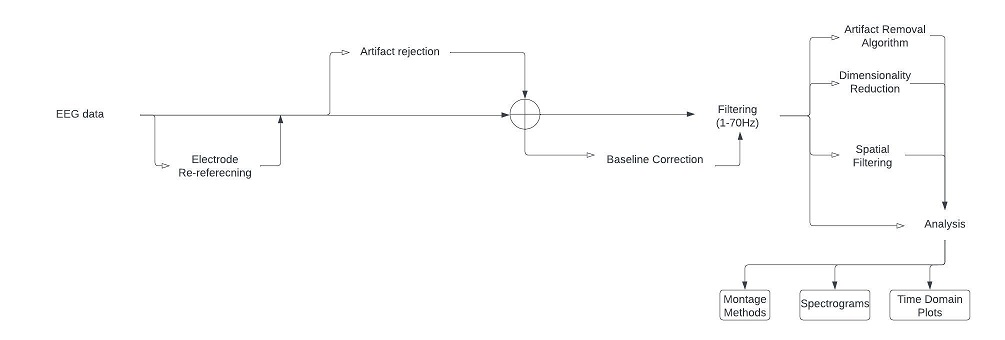
\includegraphics{preProcessing.jpeg}
  \caption{Newly Adopted preprocessing pipeline}
  \label{fig:preprocessPipeline}
\end{figure}
\begin{figure}
  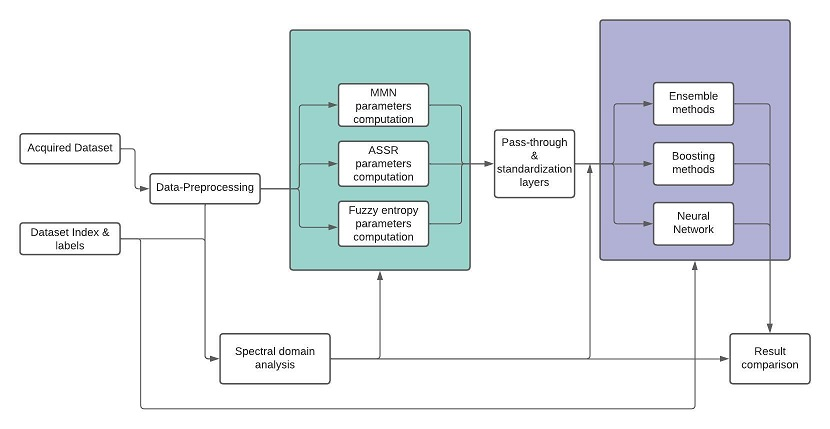
\includegraphics{workflowArchitecture.jpeg}
  \caption{Workflow Architecture}
  \label{fig:workflow Architecture}
\end{figure}

\clearpage
% \subsection{montages}
\begin{figure}
  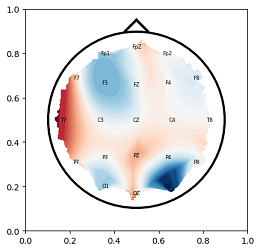
\includegraphics{ordinary_montage.png}
  \caption{Ordinary EEG Montage}
  \label{fig:ordinary eeg montage}
\end{figure}
\begin{figure}
  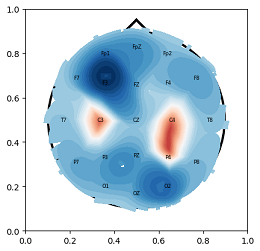
\includegraphics{edge_mean_montage.png}
  \caption{EEG Montage using Edge Interpolation}
  \label{fig:EEG montage with edge}
\end{figure}
\begin{figure}
  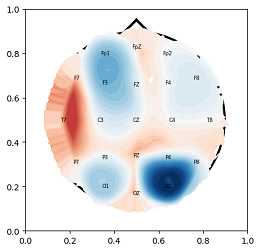
\includegraphics{edge_mean_baseline_montage.png}
  \caption{EEG Montage with baseline correction \& Edge Interpolation}
  \label{fig:EEG montage with edge and baseline correction}
\end{figure}

\begin{figure}
  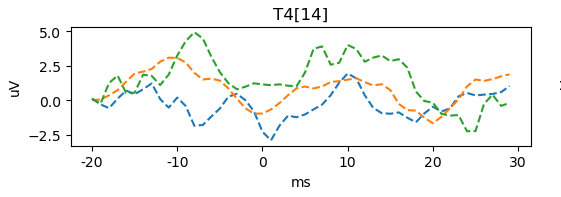
\includegraphics{simiat_temporal.png}
  \caption{Time-Series Plot(MMN) for a patient} 
  \label{fig:MMN time-series plota}
\end{figure}

\begin{figure}
  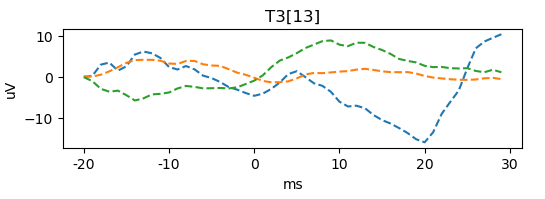
\includegraphics{simiat_temporal1.png}
  \caption{Time-Series Plot(MMN) for a patient} 
  \label{fig:MMN time-series plot}
\end{figure}

\clearpage
% \subsection{pipelines}



\begin{landscape}
	content...

\begin{figure}
  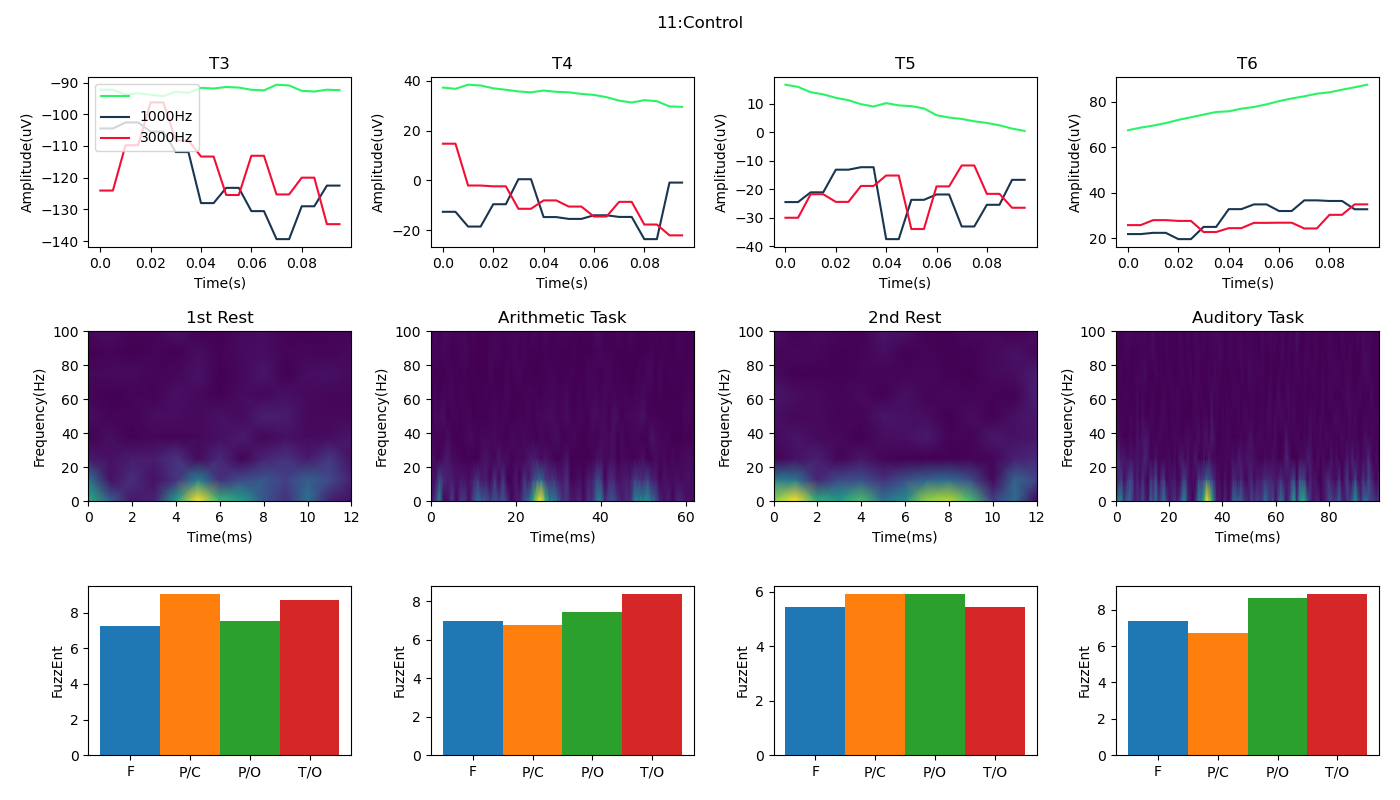
\includegraphics[width=7.2in]{figures/11.png}
  \caption{Control 11}
  \label{fig:control_11}
\end{figure}
\clearpage
\begin{figure}
  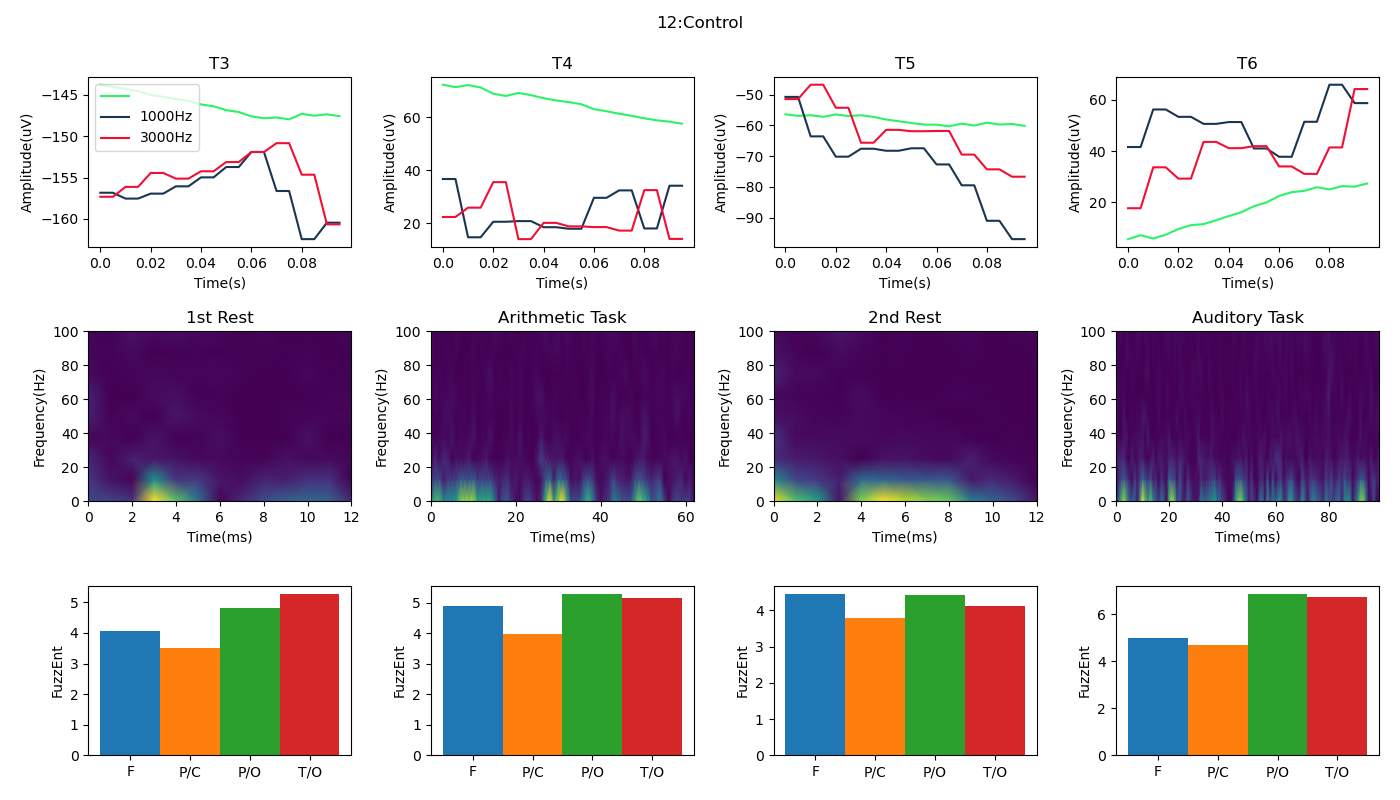
\includegraphics[width=7.2in]{figures/12.png}
  \caption{Control 12}
  \label{fig:control_12}
\end{figure}
\clearpage
\begin{figure}
  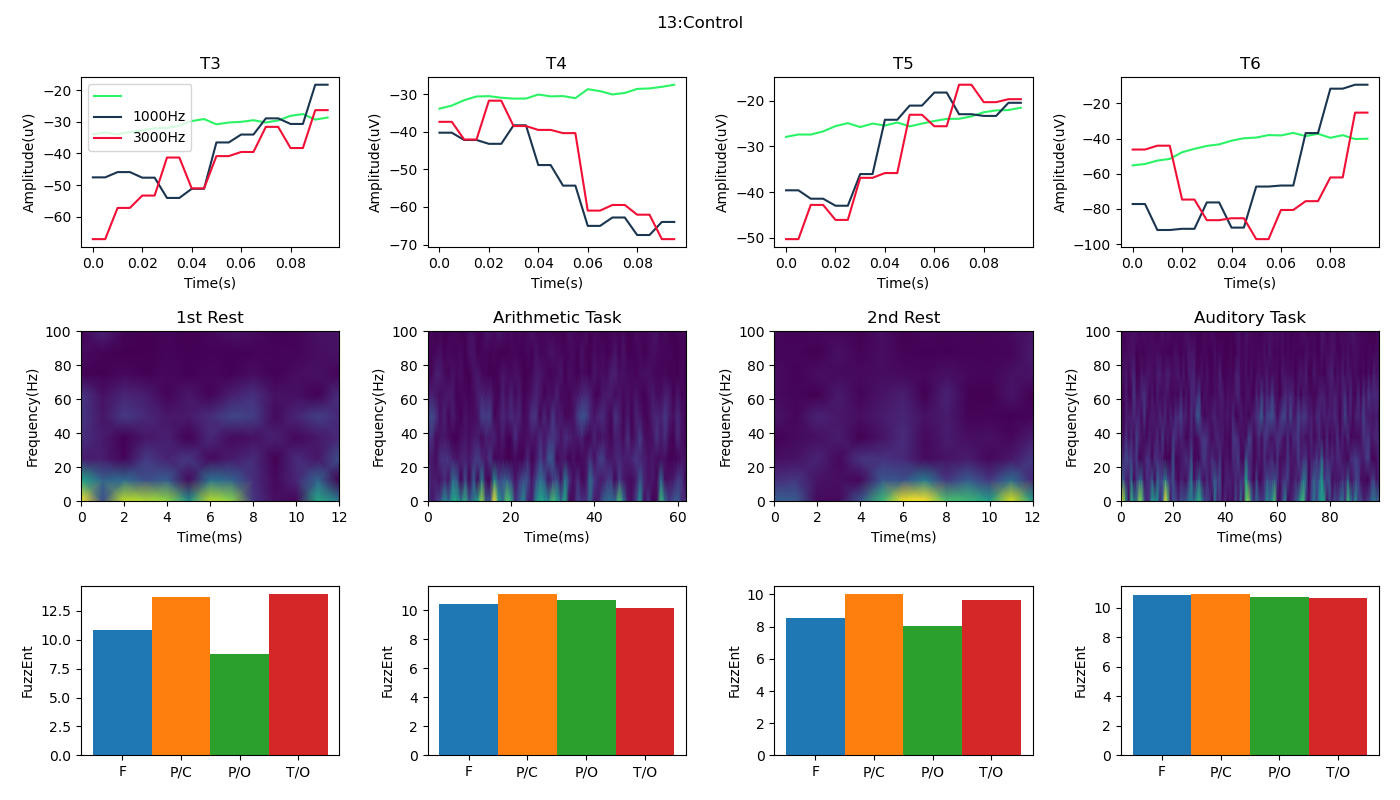
\includegraphics[width=7.2in]{figures/13.png}
  \caption{Control 13}
  \label{fig:control_13}
\end{figure}
\clearpage
\begin{figure}
  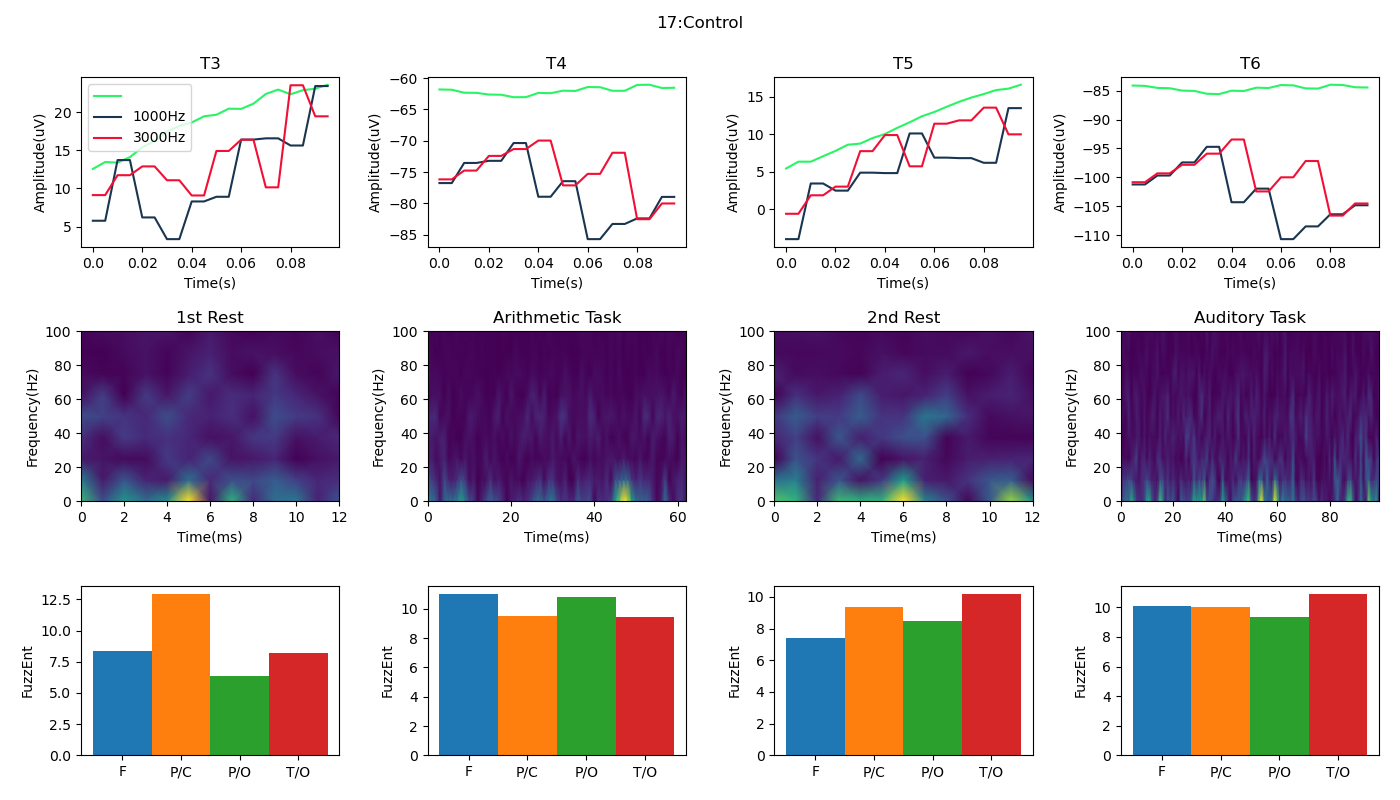
\includegraphics[width=7.2in]{figures/17.png}
  \caption{Control 17}
  \label{fig:control_17}
\end{figure}
\clearpage
\begin{figure}
  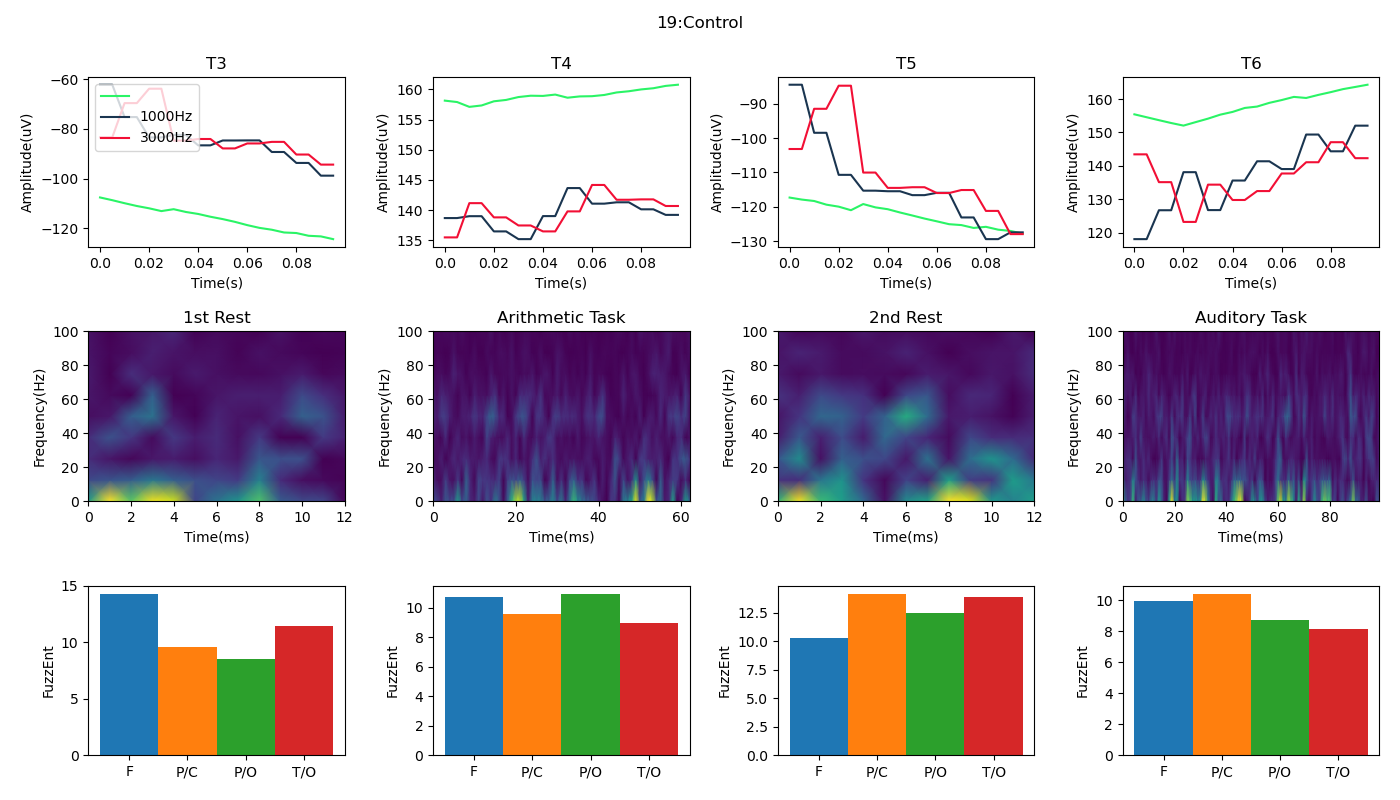
\includegraphics[width=7.2in]{figures/19.png}
  \caption{Control 19}
  \label{fig:control_19}
\end{figure}
\clearpage
\begin{figure}
  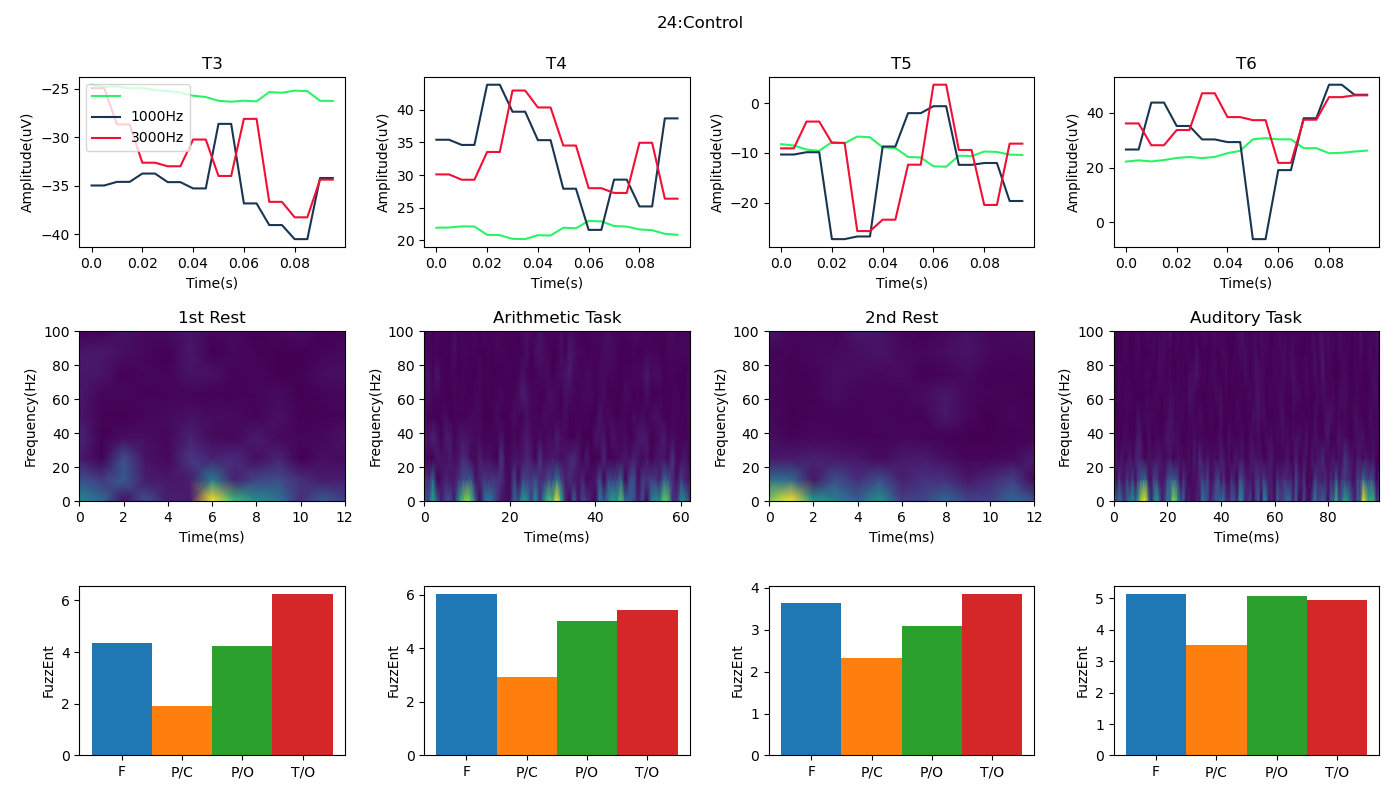
\includegraphics[width=7.2in]{figures/24.png}
  \caption{Control 24}
  \label{fig:control_24}
\end{figure}
\clearpage
\begin{figure}
  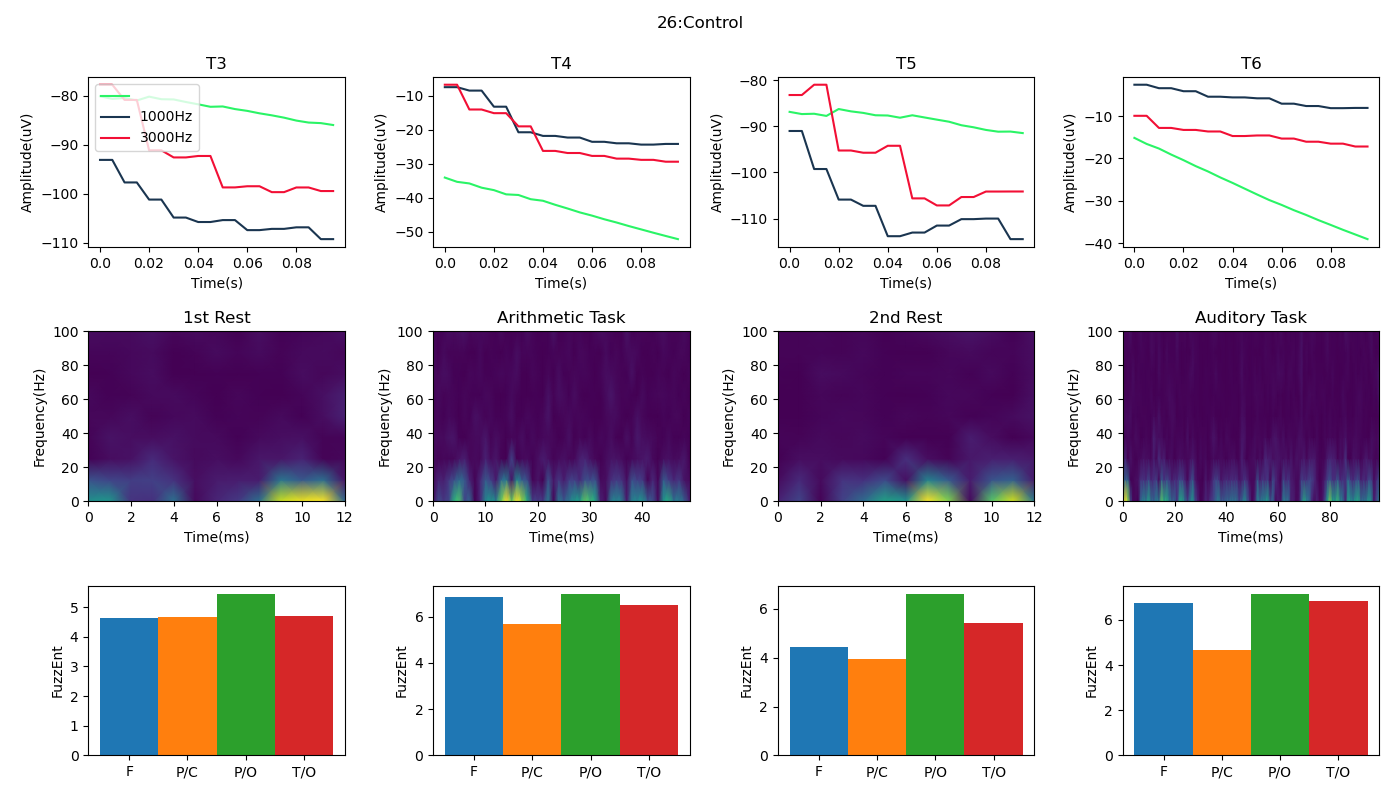
\includegraphics[width=7.2in]{figures/26.png}
  \caption{Control 26}
  \label{fig:control_26}
\end{figure}
\clearpage
\begin{figure}
  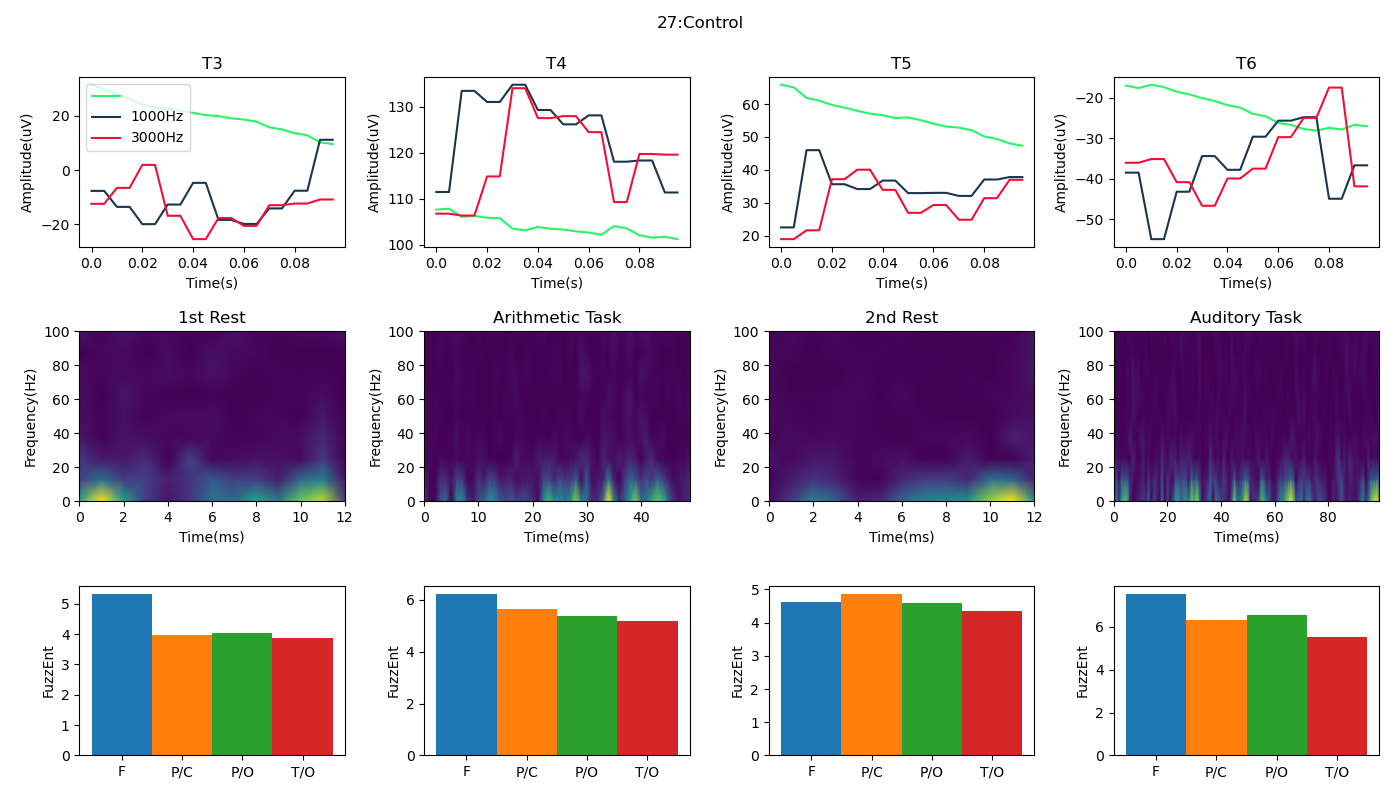
\includegraphics[width=7.2in]{figures/27.png}
  \caption{Control 27}
  \label{fig:control_27}
\end{figure}
\clearpage
\begin{figure}
  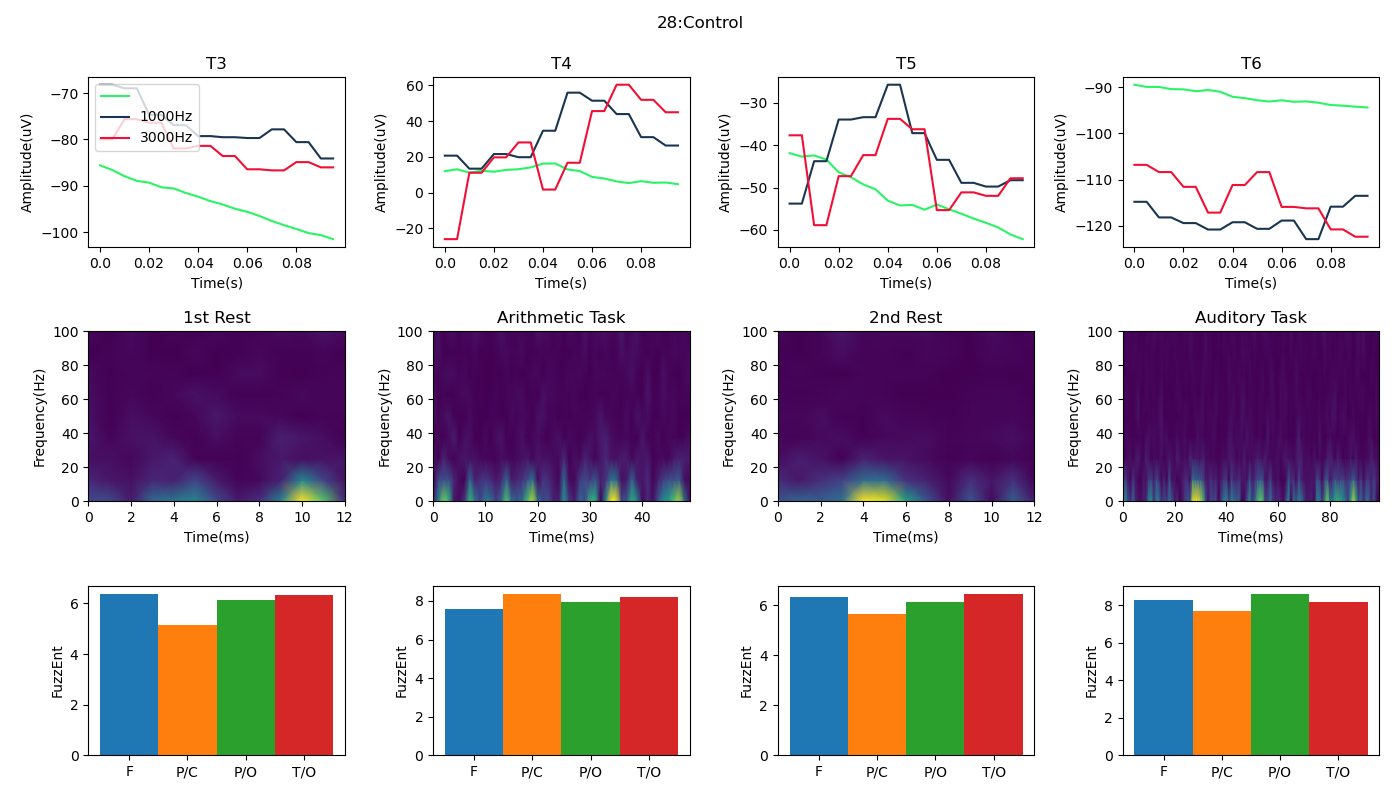
\includegraphics[width=7.2in]{figures/28.png}
  \caption{Control 28}
  \label{fig:control_28}
\end{figure}
\clearpage
\begin{figure}
  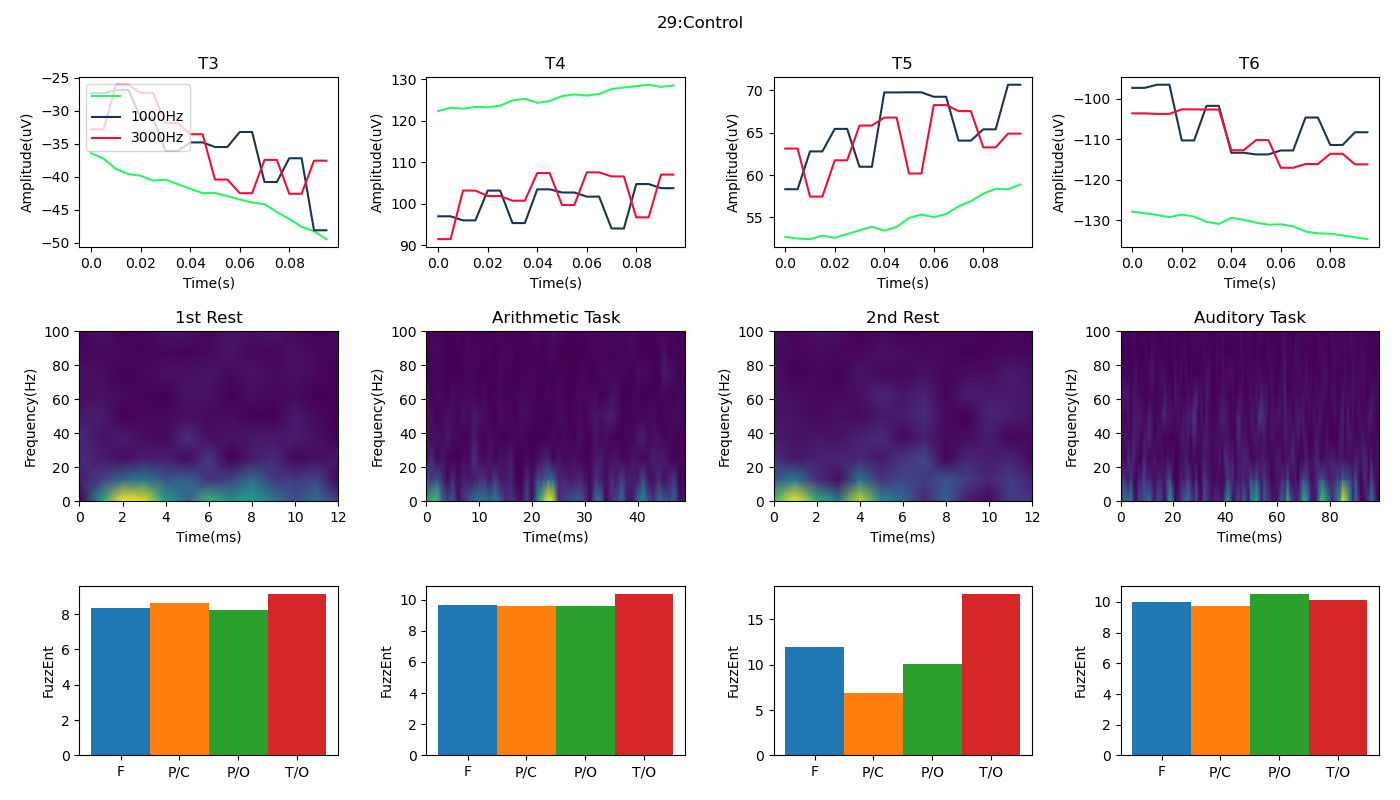
\includegraphics[width=7.2in]{figures/29.png}
  \caption{Control 29}
  \label{fig:control_29}
\end{figure}
\clearpage
\begin{figure}
  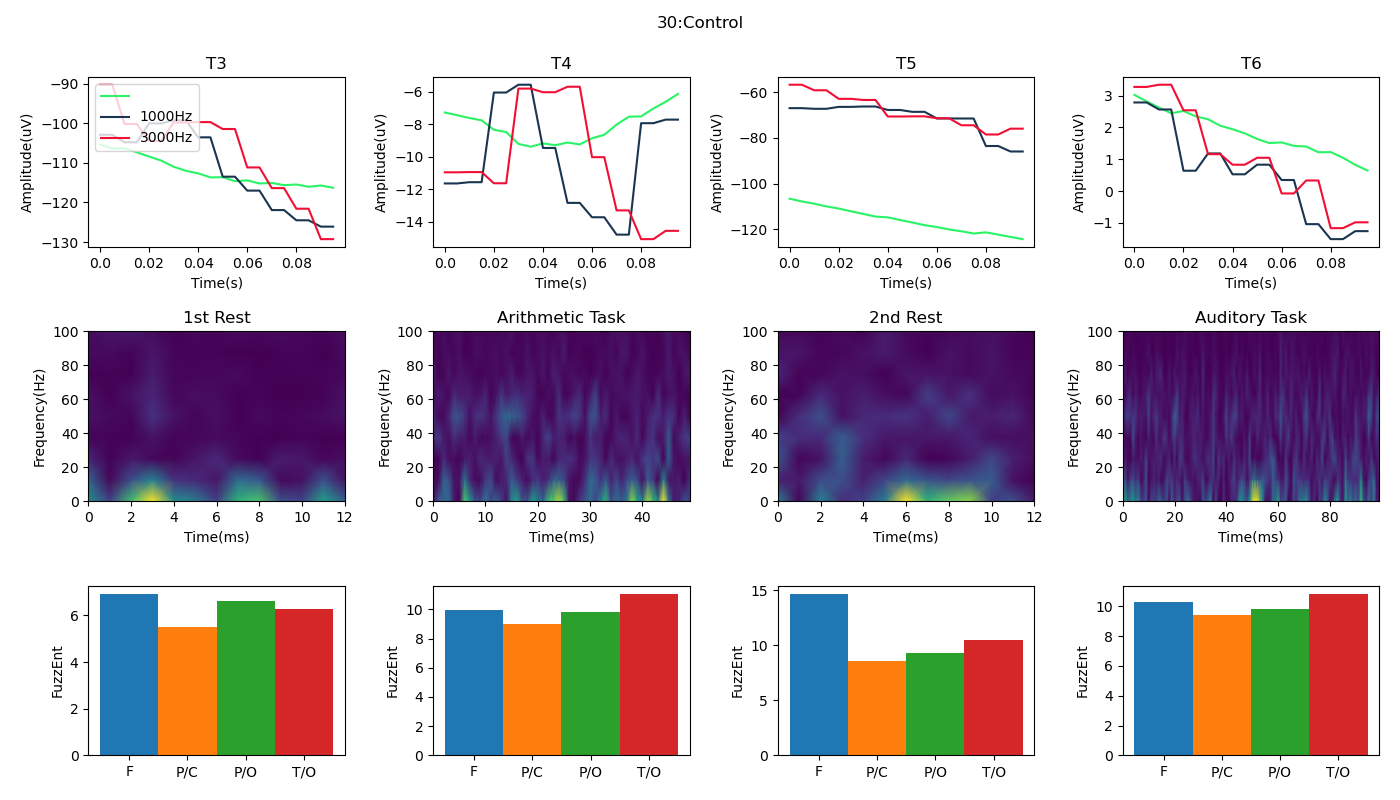
\includegraphics[width=7.2in]{figures/30.png}
  \caption{Control 30}
  \label{fig:control_30}
\end{figure}
\clearpage
\begin{figure}
  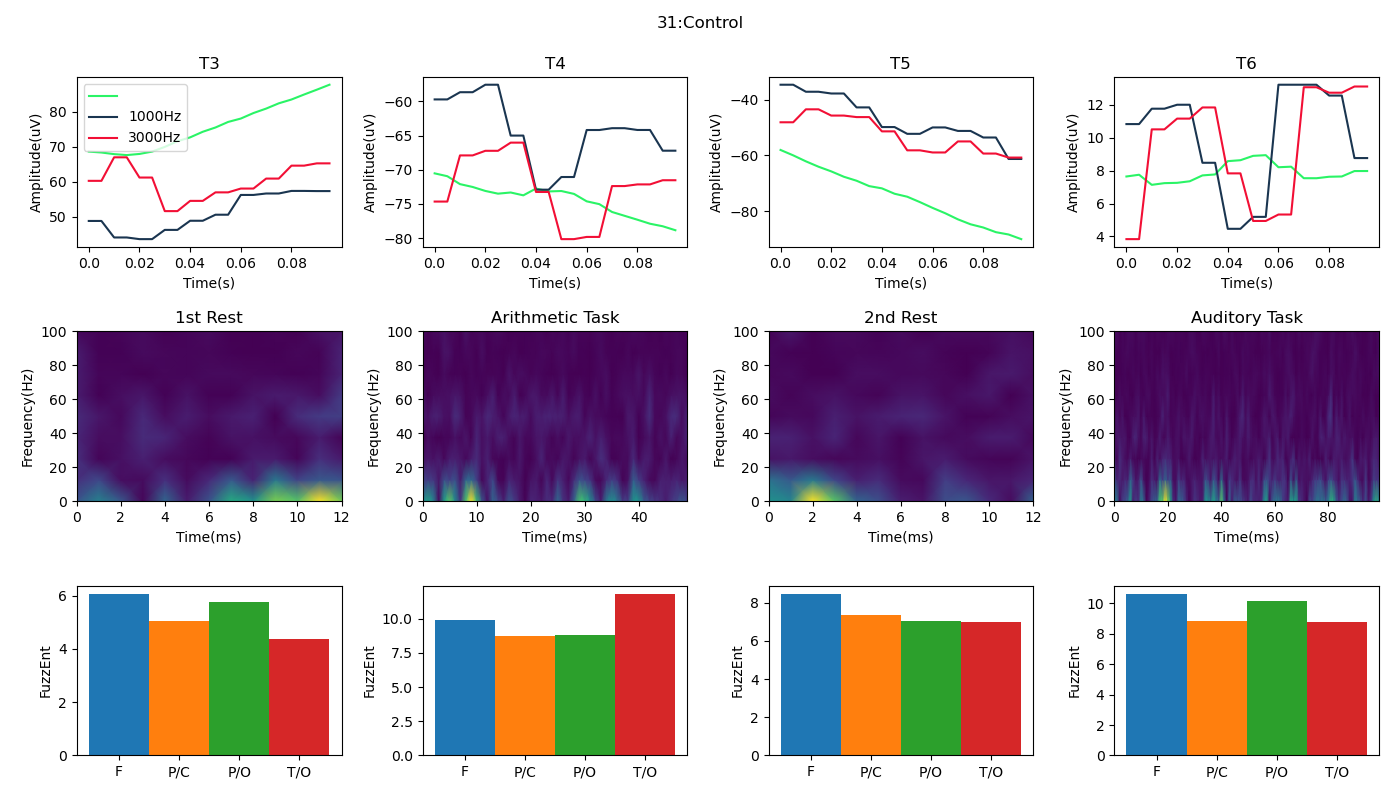
\includegraphics[width=7.2in]{figures/31.png}
  \caption{Control 31}
  \label{fig:control_31}
\end{figure}

\clearpage
\begin{figure}
  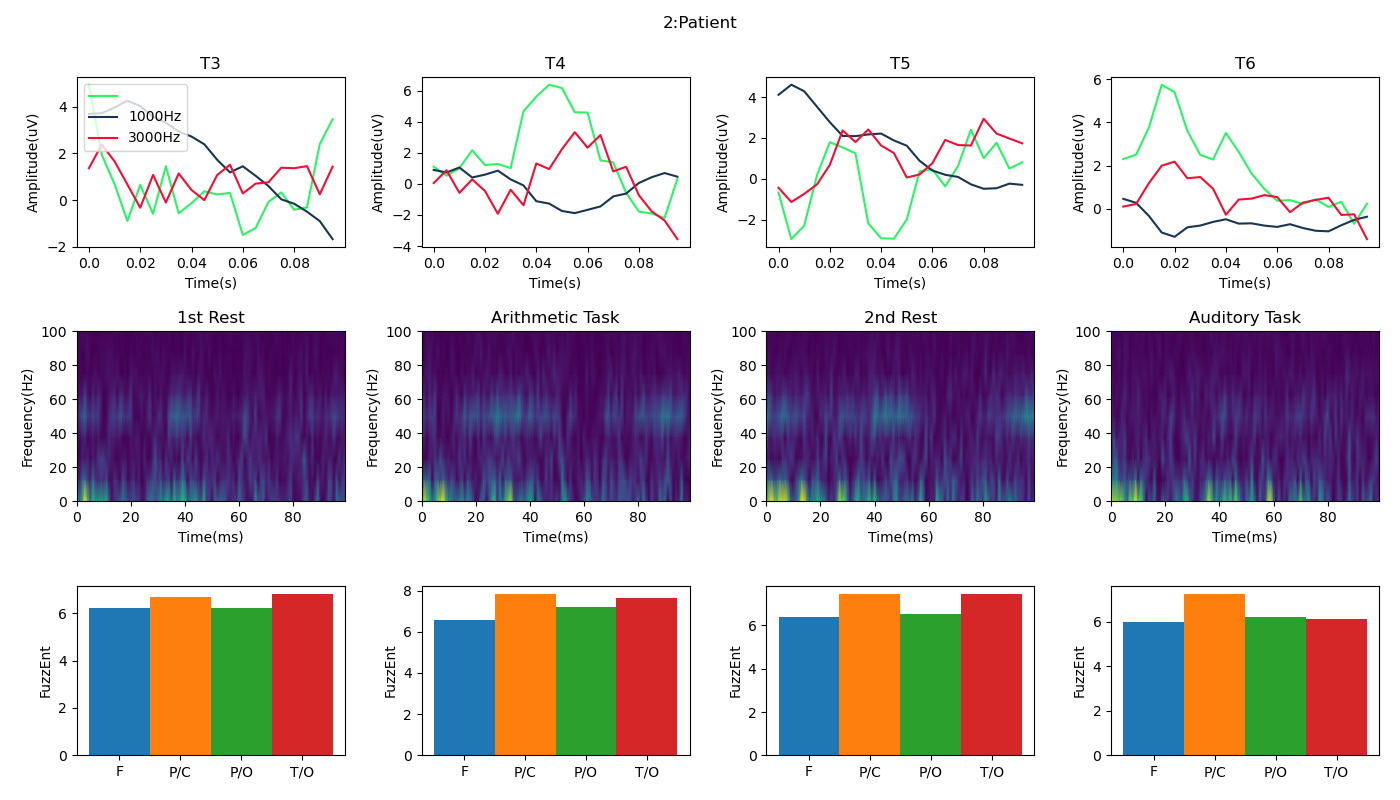
\includegraphics[width=7.2in]{figures/2.png}
  \caption{Patient 2}
  \label{fig:patient_2}
\end{figure}
\clearpage
\begin{figure}
  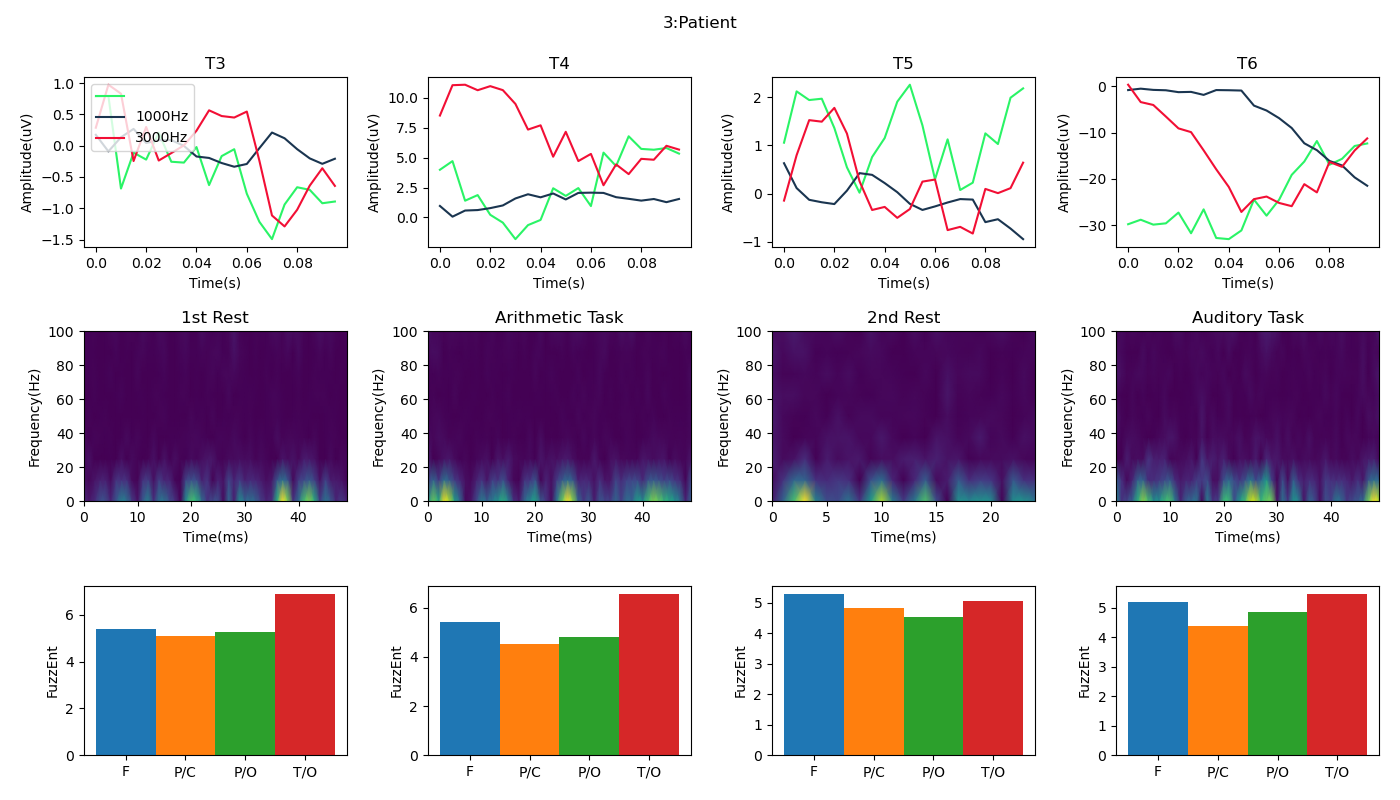
\includegraphics[width=7.2in]{figures/3.png}
  \caption{Patient 3}
  \label{fig:patient_3}
\end{figure}
\clearpage
\begin{figure}
  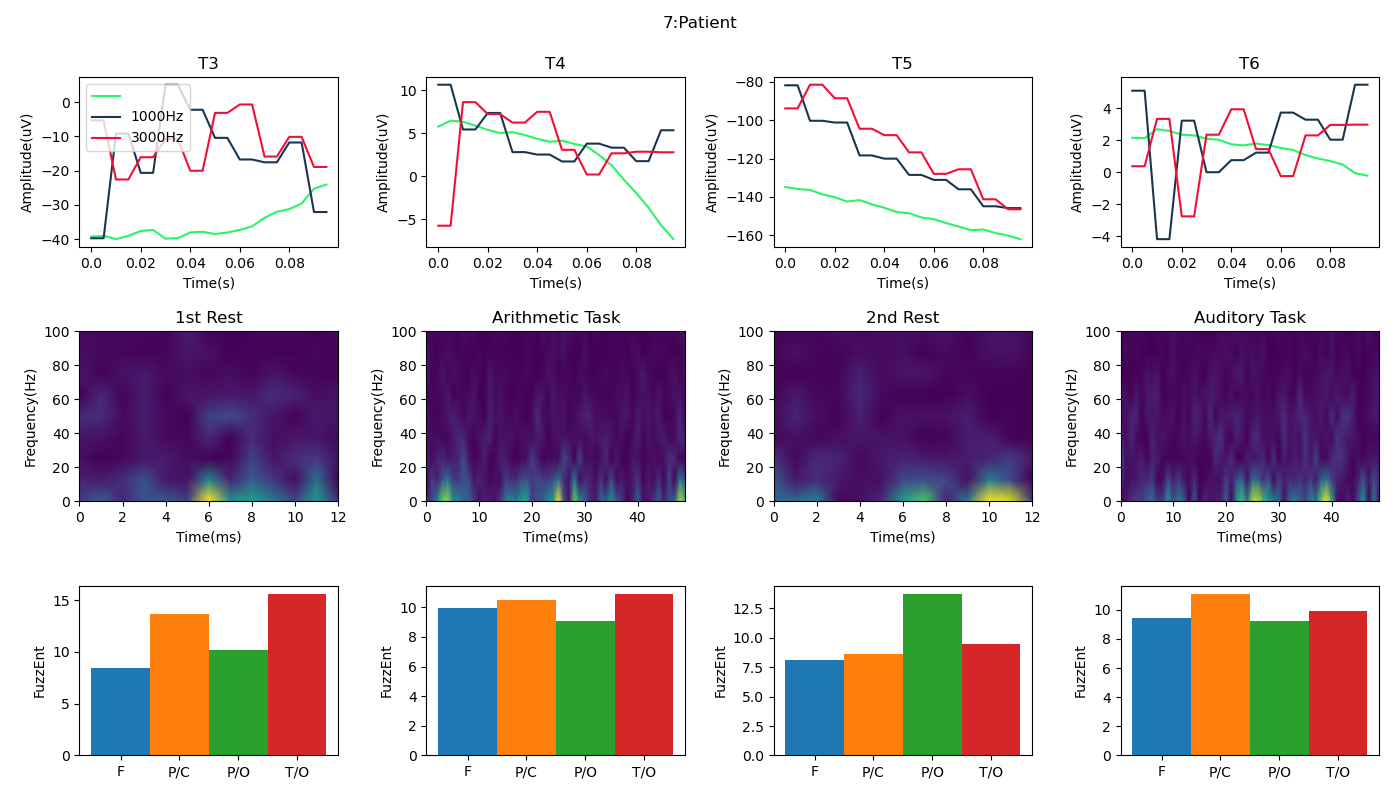
\includegraphics[width=7.2in]{figures/7.png}
  \caption{Patient 7}
  \label{fig:patient_7}
\end{figure}
\clearpage
\begin{figure}
  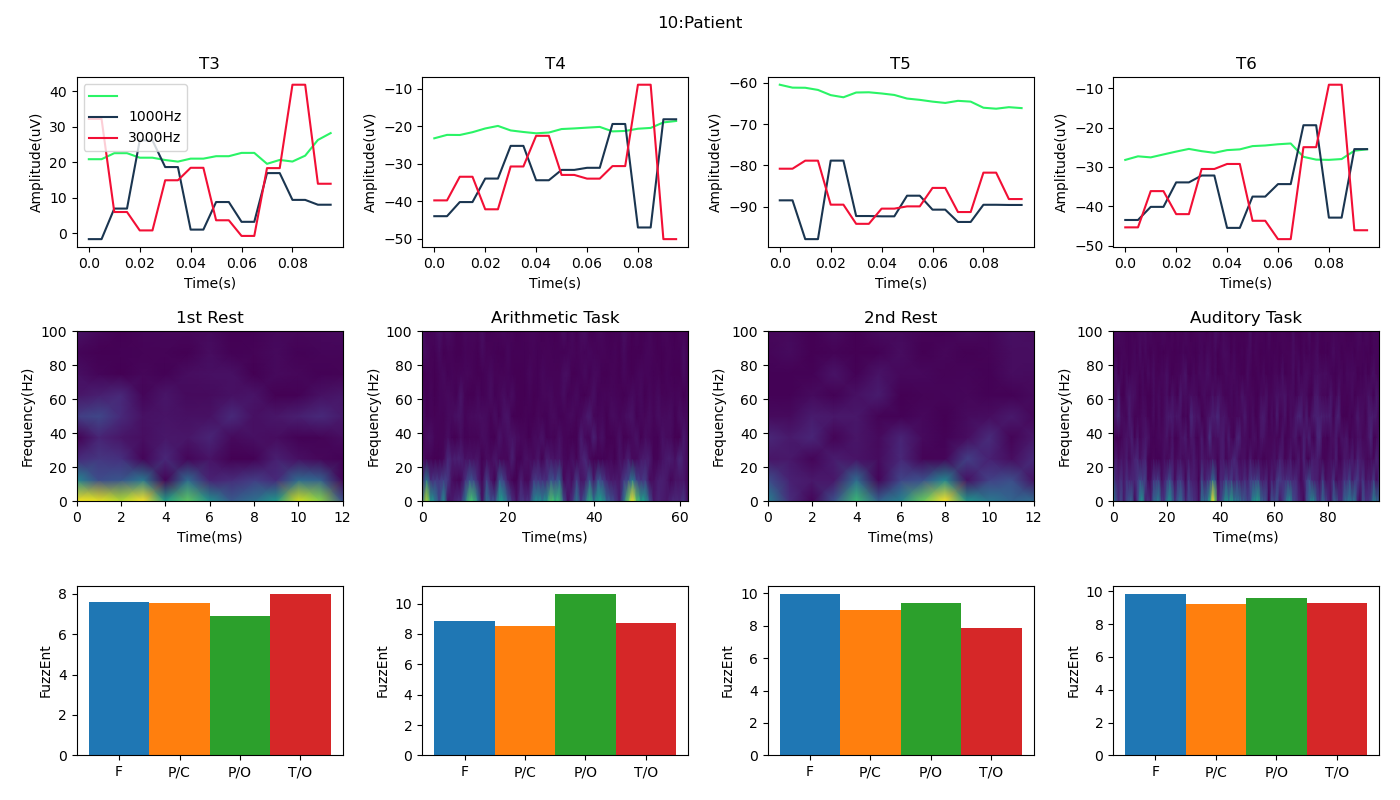
\includegraphics[width=7.2in]{figures/10.png}
  \caption{Patient 10}
  \label{fig:patient_10}
\end{figure}
\clearpage
\begin{figure}
  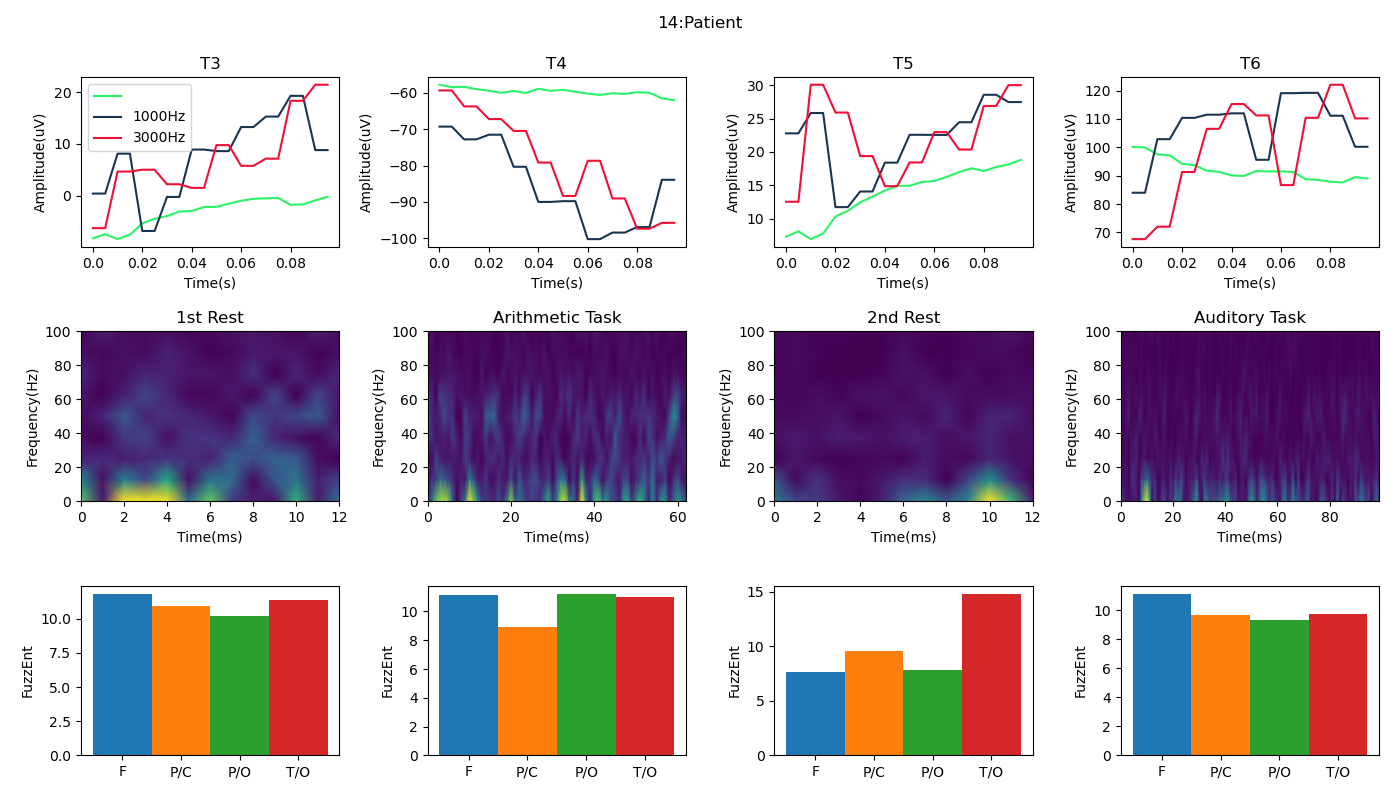
\includegraphics[width=7.2in]{figures/14.png}
  \caption{Patient 14}
  \label{fig:patient_14}
\end{figure}
\clearpage
\begin{figure}
  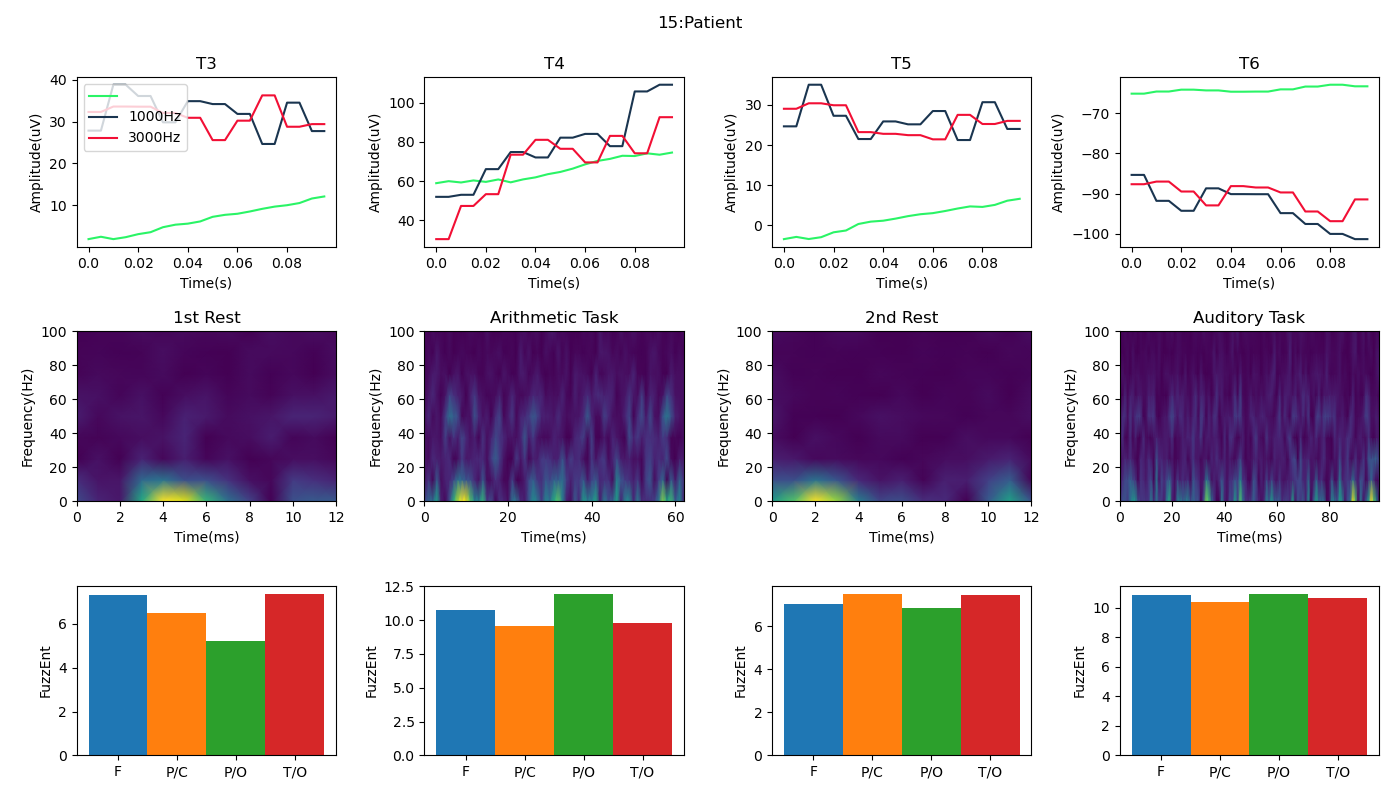
\includegraphics[width=7.2in]{figures/15.png}
  \caption{patient 15}
  \label{fig:patient_15}
\end{figure}
\clearpage
\begin{figure}
  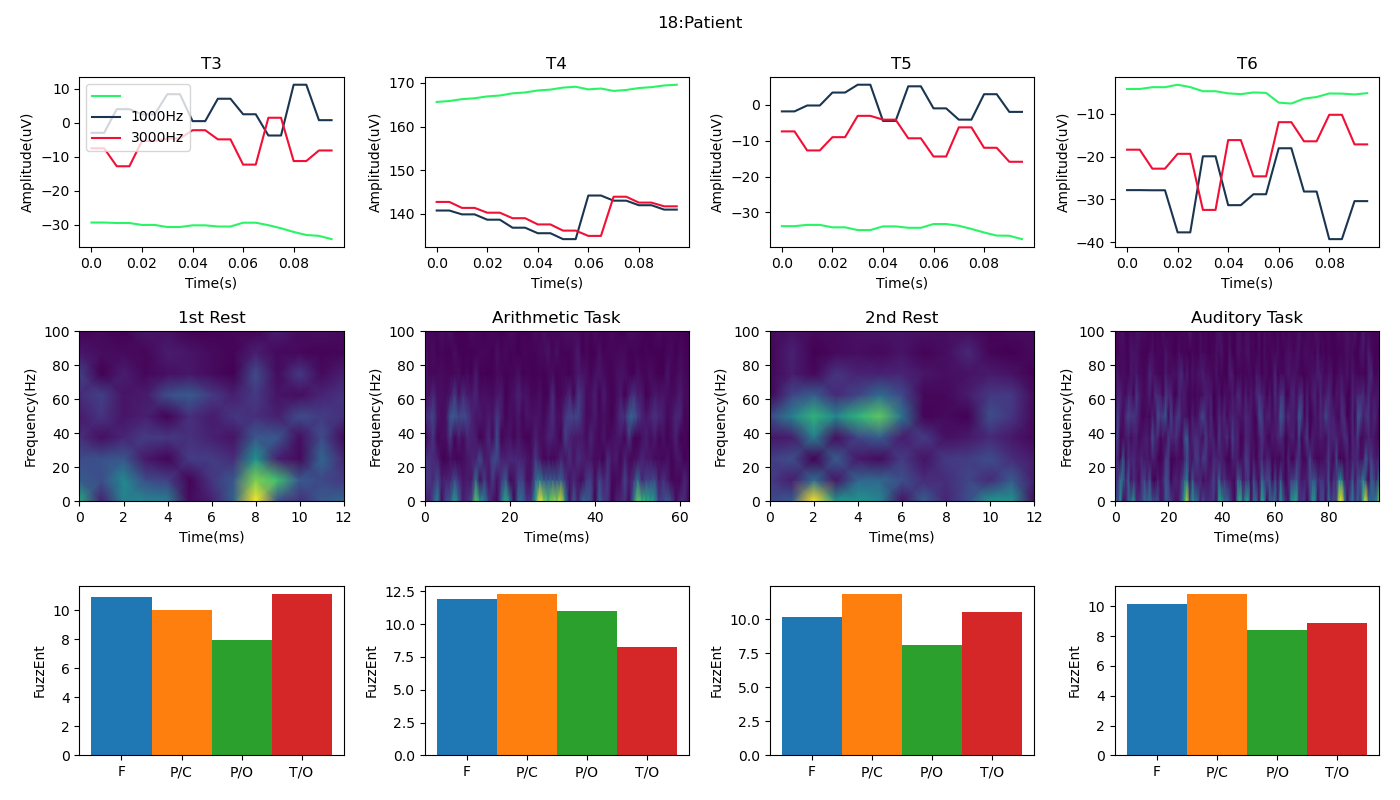
\includegraphics[width=7.2in]{figures/18.png}
  \caption{patient 18}
  \label{fig:patient_18}
\end{figure}
\clearpage
\begin{figure}
  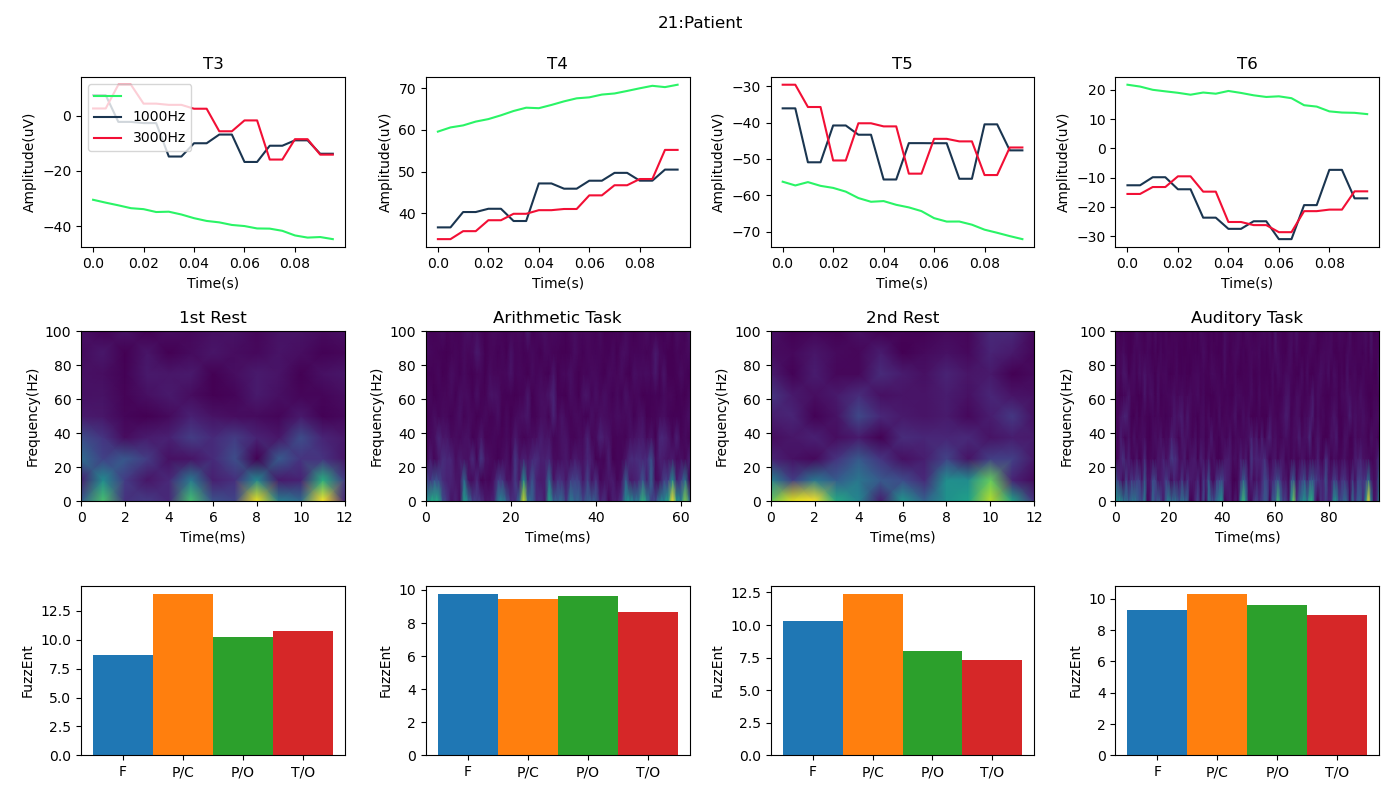
\includegraphics[width=7.2in]{figures/21.png}
  \caption{patient 21}
  \label{fig:patient_21}
\end{figure}
\clearpage
\begin{figure}
  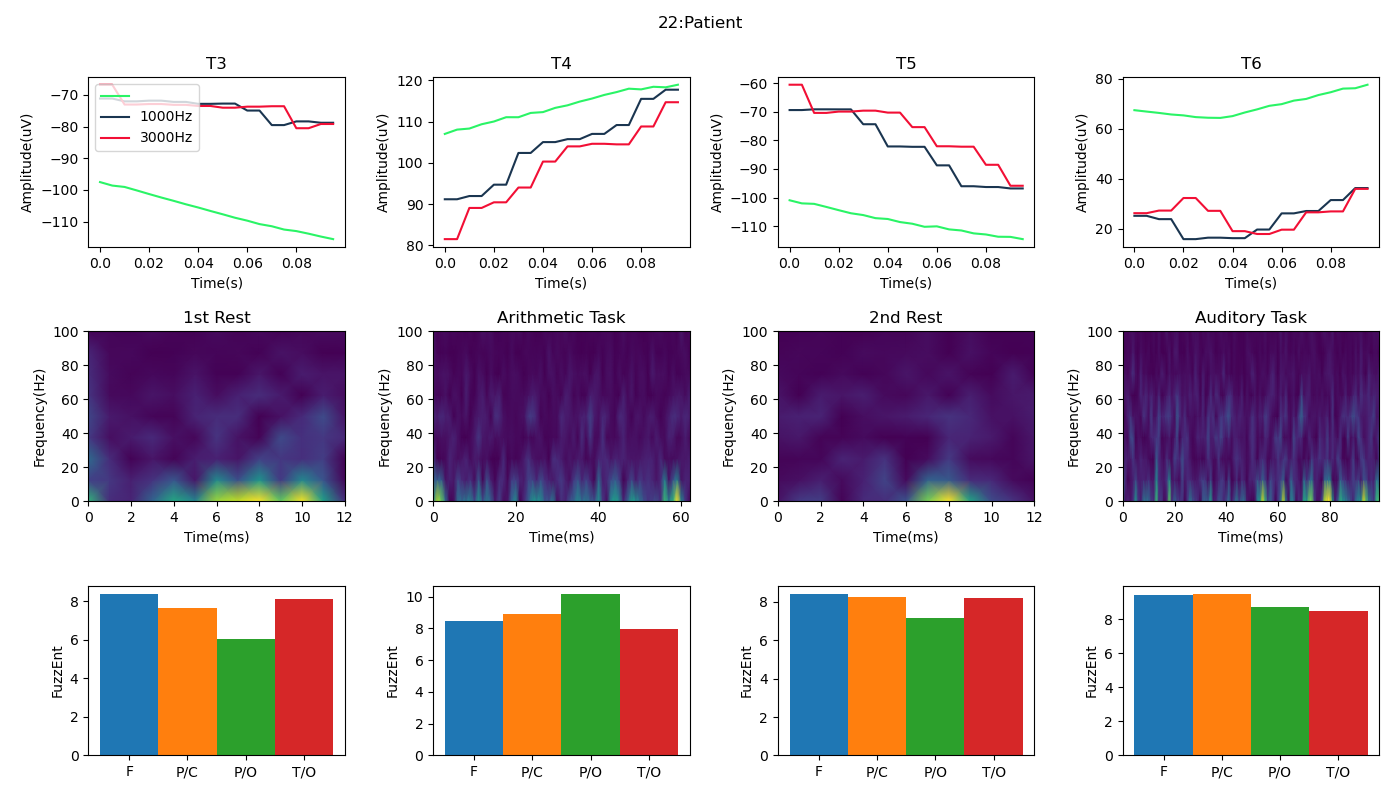
\includegraphics[width=7.2in]{figures/22.png}
  \caption{Patient 22}
  \label{fig:patient_22}
\end{figure}
\clearpage
\begin{figure}
  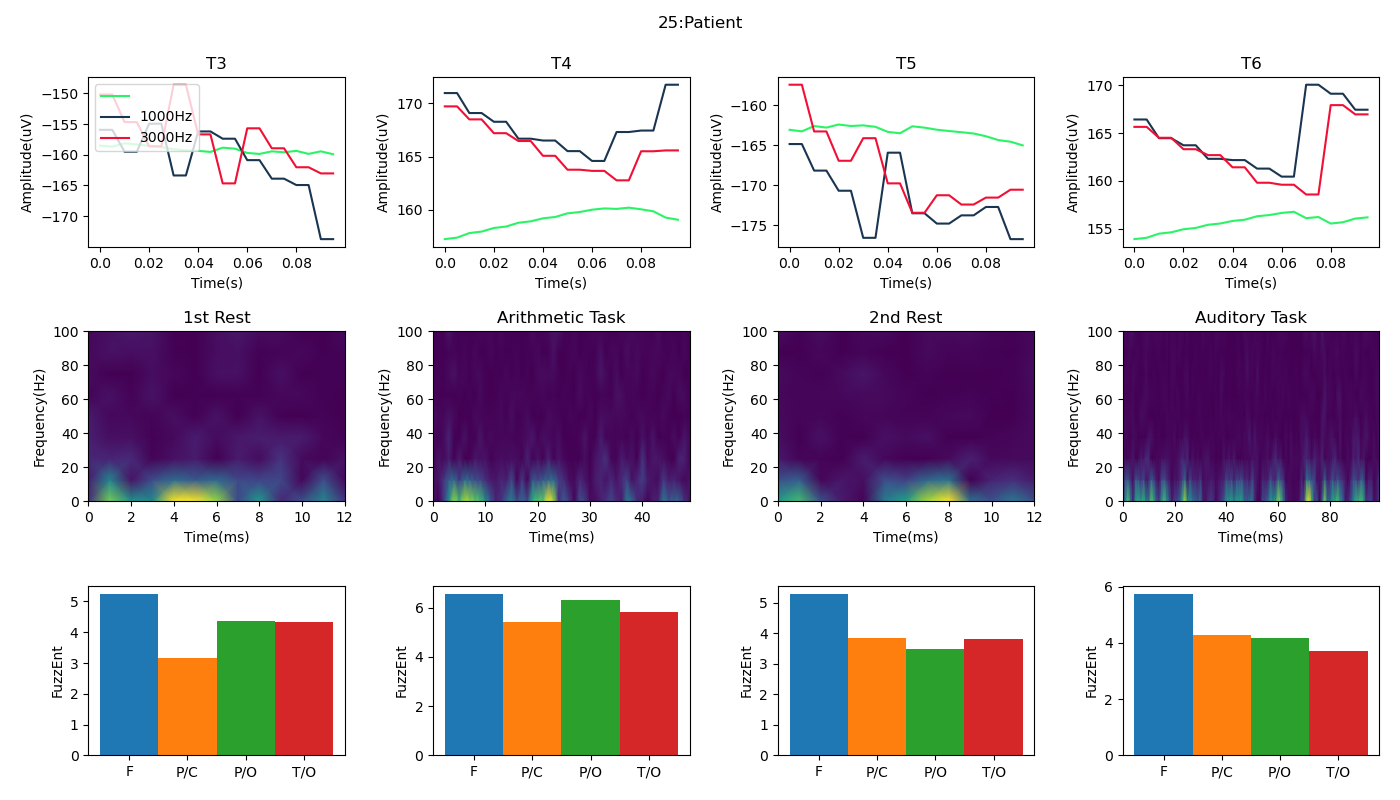
\includegraphics[width=7.2in]{figures/25.png}
  \caption{Patient 25}
  \label{fig:patient_25}
\end{figure}
\end{landscape}


\end{document}